\documentclass[10pt,a4paper]{article}
\usepackage[margin=22mm]{geometry}
\usepackage[T1]{fontenc}
\usepackage{lmodern}
\usepackage{microtype}
\usepackage{graphicx}
\usepackage{booktabs}
\usepackage{longtable}
\usepackage{array}
\usepackage{enumitem}
\usepackage{xcolor}
\usepackage{hyperref}
\usepackage{url}
\usepackage{caption}
\usepackage{authblk}
\usepackage{float}
\hypersetup{colorlinks=true,linkcolor=black,citecolor=black,urlcolor=blue}
\setlist{nosep,leftmargin=*}
\setlist[description]{style=multiline,leftmargin=4.9cm,labelwidth=4.4cm,labelsep=0.35cm}
\newcommand{\code}[1]{\texttt{#1}}
\newcommand{\placeholder}[1]{\textbf{[#1]}}

\title{A version-paired dataset of dependency and interface evolution in Python research software}
\author[1,*]{Yanbo Bian}
\author[1,*]{Zhihai Wang}
\affil[1]{Beijing Jiaotong University, Beijing 100044, China\\
\href{mailto:24722081@bjtu.edu.cn}{24722081@bjtu.edu.cn};
\href{mailto:zhhwang@bjtu.edu.cn}{zhhwang@bjtu.edu.cn}}
\affil[*]{Correspondence to Yanbo Bian or Zhihai Wang.}
\date{}

\begin{document}
\maketitle

\begin{abstract}
Research software is cited through papers while repositories change. We release a version-paired static dataset linking the immutable archive associated with a Journal of Open Source Software (JOSS) article to a later immutable GitHub endpoint. It covers 345 Python projects from JOSS articles published in 2018--2020, represented by 690 source snapshots. The release contains 9,074 declared-dependency records, 121,085 syntactic-interface records, 95,787 evidence-linked pair-delta records and 2,876 validation records, plus project, snapshot and structure metadata. Endpoints were resolved on 14 August 2026: 327 stable releases and 18 default-branch commits. Extraction is static; candidate software was not installed, imported or executed. The tables support studies of dependency, source-level interface, packaging, Python-version, project-structure and parser changes. Syntactic differences are not runtime compatibility, declarations are not resolved environments, and summaries are not quality or population-prevalence estimates.\footnote{The formal dataset DOI and DOI-minted archive of the tagged code release are marked explicitly in this manuscript and must be completed before submission.}
\end{abstract}

\section*{Background \& Summary}

Research software is part of the scholarly record, but a software article and its linked repository provide different temporal anchors. The article fixes a citable publication context, whereas the repository may be renamed, archived or modified after publication. A reuser who wants to study how a research tool was declared, exposed or documented therefore needs a source snapshot tied to publication and a later snapshot whose identity is immutable. Persistent software identifiers and citation practices provide the provenance rationale for such a record, while FAIR principles require machine-readable metadata and stable access paths \cite{soito2017software,wilkinson2016fair}.

Several public resources address complementary parts of this problem. OpenDORS links more than 134,000 open research-software projects to publications and supplies repository-level metadata \cite{druskat2025opendors}; SemRepo connects research repositories to scholarly knowledge graphs \cite{rafay2026semrepo}; and the Software Heritage Graph provides broad source-history infrastructure \cite{pietri2019softwareheritage}. Other datasets describe dependency networks, workflow histories, research-code execution, static-analysis reports or source-derived code-smell records \cite{schueller2022rust,cardoen2024actions,trisovic2022researchcode,koszo2025static,alomari2025smellycode}. These resources establish the value of reusable software traces, but their released units do not provide the same project-level object: a publication-linked immutable archive paired with a later immutable endpoint and accompanied by evidence-bearing field deltas across dependency, interface and project-structure families.

We constructed this paired resource from the frozen Crossref frame of JOSS articles with publication dates from 1 January 2018 through 31 December 2020. Each retained project is linked to an immutable publication archive associated with the article and to the latest non-draft, non-prerelease GitHub release available on 14 August 2026. The paired cohort contains 341 Zenodo and 4 Figshare publication snapshots. When no qualifying release was available, the endpoint is the default-branch head resolved to a full commit SHA. The static pipeline records archive identity and checksums, parser versions, relative source evidence, missingness and validation events. It never installs, imports or executes third-party code.

The resulting data object supports field-level analyses of declared dependency changes, Python-version and packaging metadata, syntactic surface changes, test and continuous-integration configuration, scholarly metadata files and parser behavior. It is a bounded JOSS/Python census rather than a representative sample of research software. Its records describe observable source and metadata states; they do not establish runtime compatibility, installability, maintenance quality, sustainability, causal explanations for change or population-wide prevalence.

\section{Methods}

\subsection{Study design and unit of observation}

The resource is organized around a project-level pair. A \code{project\_id} is derived from the normalized JOSS DOI, a \code{pair\_id} identifies the two snapshots, and each child row retains its parent \code{snapshot\_id} or \code{pair\_id}. A resolved project therefore has exactly one publication snapshot and one endpoint snapshot. Unresolved endpoint projects remain in the selection and endpoint ledgers but produce no fabricated snapshot or delta rows. This design makes provenance and missingness part of the data object rather than post hoc exclusions.

\subsection{Frame construction and deterministic screening}

The source frame was acquired from the Crossref journal works endpoint for ISSN 2475-9066 and the date interval above. The frozen frame contains 940 records. DOIs were normalized to lowercase and assigned a deterministic SHA-256 rank using the frozen screening salt. The rank controlled processing order only; it was not a sampling weight or eligibility feature. Every frame record was retained in a screening ledger with its status and reason code.

Metadata screening required a declared GitHub repository that was not identified as a fork, exposed a default branch, contained root-level Python packaging evidence and reported a machine-confirmed licence identifier. Of the 940 records, 396 passed these checks, 537 were excluded with explicit reason codes and 7 remained unresolved after official-source checks. The subsequent publication-archive audit retained 372 archive-eligible projects, excluded 20 and left 4 unresolved. Endpoint resolution was attempted for all 372 archive-eligible projects; 345 resolved and 27 remained unresolved. The 345 resolved projects form the paired extraction cohort. Explicit frame, eligibility and attrition records make the cohort boundary available for repository-mining analyses \cite{robredo2024cohort}.

\subsection{Scholarly linkage and publication snapshots}

The workflow retained the JOSS DOI, article metadata, article URL and declared repository URL. Repository redirects and renames were represented by both input and canonical URLs. Publication snapshots were selected from immutable software-archive records linked to the articles. The final paired cohort uses 341 Zenodo records and 4 Figshare records. When multiple files were present, a source tar archive was preferred, then a source ZIP; built wheels were lower priority. The selected archive DOI, file key, source URL, upstream checksum, locally computed SHA-256, byte size and parser version were recorded in \code{snapshot\_records.csv}. Publication archives were checked against their provider-reported MD5 values as well as the local SHA-256.

\subsection{Endpoint policy and immutable acquisition}

Endpoint selection followed a frozen release-or-commit policy. The resolver selected the latest GitHub release that was neither draft nor prerelease. If no such release existed, it selected the default-branch head. The selected reference was resolved to a 40-character commit SHA, and the source archive was addressed by that SHA rather than by a mutable branch or tag URL. Among the 345 resolved endpoints, 327 were releases and 18 were default-branch heads. Eighty-three resolutions used the GitHub REST API and 262 used official GitHub web surfaces because the unauthenticated API was rate limited. The resolution method, evidence URLs, reference, commit and archive checksum are retained in the endpoint ledger and snapshot table. The 27 unresolved projects retain their official-source failure states.

\subsection{Bounded static archive access}

ZIP and TAR members were read with Python archive readers without extraction to runnable locations. Absolute paths, drive-prefixed paths and path-traversal members were flagged; symbolic and hard links were counted but not followed; common wrapper directories and platform-generated \code{\_\_MACOSX} members were removed. The archive reader enforced limits of 100,000 members, 2 MiB per selected text member and 128 MiB of selected text per archive. Candidate modules and build scripts were parsed as data. In particular, \code{setup.py} was inspected syntactically and never executed.

\subsection{Dependency, interface and structure extraction}

Declared direct dependencies were parsed from PEP 621 and Poetry sections in \code{pyproject.toml}, PEP 517 build requirements, \code{setup.cfg}, statically readable arguments to \code{setup()}, requirements files and conda environment files. Python dependency extraction depends on both the observable source evidence and the extraction method \cite{jin2024pyanalyzer}; each observation therefore preserves its source file, parser kind, dependency group, normalized name, raw declaration, specifier, marker, extras and parse status. Overlapping declaration files are retained as separate evidence; the table is not a dependency solver output.

The interface parser selected Python source files using the documented source-root and exclusion rules. It recorded non-private top-level functions and classes, methods and constructors, normalized syntactic signatures, decorators, inferred module paths and one-based source locations. Literal \code{\_\_all\_\_} declarations were preserved as export evidence when available; otherwise the record uses the \code{lexical\_nonprivate} heuristic. Tests, examples, documentation, benchmarks, vendored directories and build directories were excluded. The result is a reproducible syntactic surface, not a runtime export or compatibility contract.

Structural extraction records packaging and build files, declared Python constraints, source-file and source-line counts, test-file counts, CI providers and workflow files, licence and citation metadata, CodeMeta and Zenodo files, changelog, contribution guide, code of conduct and security-policy presence. Presence is a binary observation of a file or configuration path and does not imply content quality or compliance.

\subsection{Pairwise comparison and descriptive summaries}

Dependency, interface and structure observations were normalized into family-specific comparison keys. For each key, \code{pair\_delta\_records.csv} stores the publication value, endpoint value, relative evidence and one of \code{added}, \code{removed}, \code{changed}, \code{unchanged} or \code{unavailable}. \code{comparison\_status} distinguishes comparable, partial-parse and unavailable records. Aggregated counts were regenerated from these rows. Descriptive summaries use the project as the aggregation unit, report no significance tests and make no causal inference. For six scalar metrics, endpoint-minus-publication medians and 95\% percentile intervals were obtained from 2,000 nonparametric project-level bootstrap resamples with seed 20260814.

\section{Data Records}

The release candidate contains seven UTF-8 CSV core tables, JSON manifests, schemas, controlled vocabularies, selection and endpoint ledgers, validation reports, summary tables and figure source data. Empty strings mean that an upstream value was unavailable or not applicable; they are not imputed zeros or false values. JSON-valued cells use sorted keys and no insignificant whitespace.

\begin{description}
\item[\texttt{project\_records.csv}] One row per scholarly project and resolved version pair, including DOI, publication date, repository identities, selection state, archive DOI, endpoint policy and endpoint reference.
\item[\texttt{snapshot\_records.csv}] Two rows per resolved project, with snapshot role, source provider, source reference, commit when known, source URL, archive bytes, SHA-256, upstream checksum and parser version.
\item[\texttt{structure\_records.csv}] One structural summary per snapshot, including packaging, archive safety, source metrics, Python constraints, tests, CI, scholarly metadata and parser completeness.
\item[\texttt{dependency\_records.csv}] Source-qualified direct dependency declarations with parser kind, group, normalized package name, raw declaration, specifier, marker, extras and parse status.
\item[\texttt{api\_symbol\_records.csv}] Syntactic functions, classes, methods and constructors with module, qualified name, normalized signature, decorators, export evidence and source locations.
\item[\texttt{pair\_delta\_records.csv}] Evidence-linked comparisons across the API, dependency and structure families. Each row is keyed by \code{pair\_id}, family, feature group and feature key.
\item[\texttt{validation\_records.csv}] Machine validation events, including archive hashes and paths, metadata parsing, AST warnings, parser errors, duplicate checks and referential-integrity checks.
\end{description}

The accompanying \code{extraction\_manifest.json} records schema and parser versions, row counts and table hashes. The endpoint-resolution manifest records the endpoint date, policy outcomes, methods and input hashes. Summary tables provide selection attrition, endpoint types, family-level project summaries, parsing completeness, paired scalar changes, project metrics and large-project sensitivity. \nolinkurl{census_overview_source_data.csv} is the source-data derivative for Fig.~\ref{fig:overview}; it is regenerated from the validated JSON and summary tables. Raw third-party source archives are not redistributed; their archive DOI or immutable commit and checksum are retained so that users can reacquire them under the original terms.

\section{Data Overview}

The 345 paired projects yield 690 snapshots, 9,074 dependency observations, 121,085 syntactic interface observations, 95,787 pair-delta rows and 2,876 validation rows. At the project level, the median endpoint-minus-publication change is 193 selected Python source lines (95\% descriptive percentile interval 87--370) and 3 syntactic interface symbols (interval 1--7). Median changes are zero for source-file count, declared dependency-record count, test-file count and CI workflow-file count. These summaries describe the observed release candidate and are not tests of a temporal effect.\par

\begin{figure}[H]
  \centering
  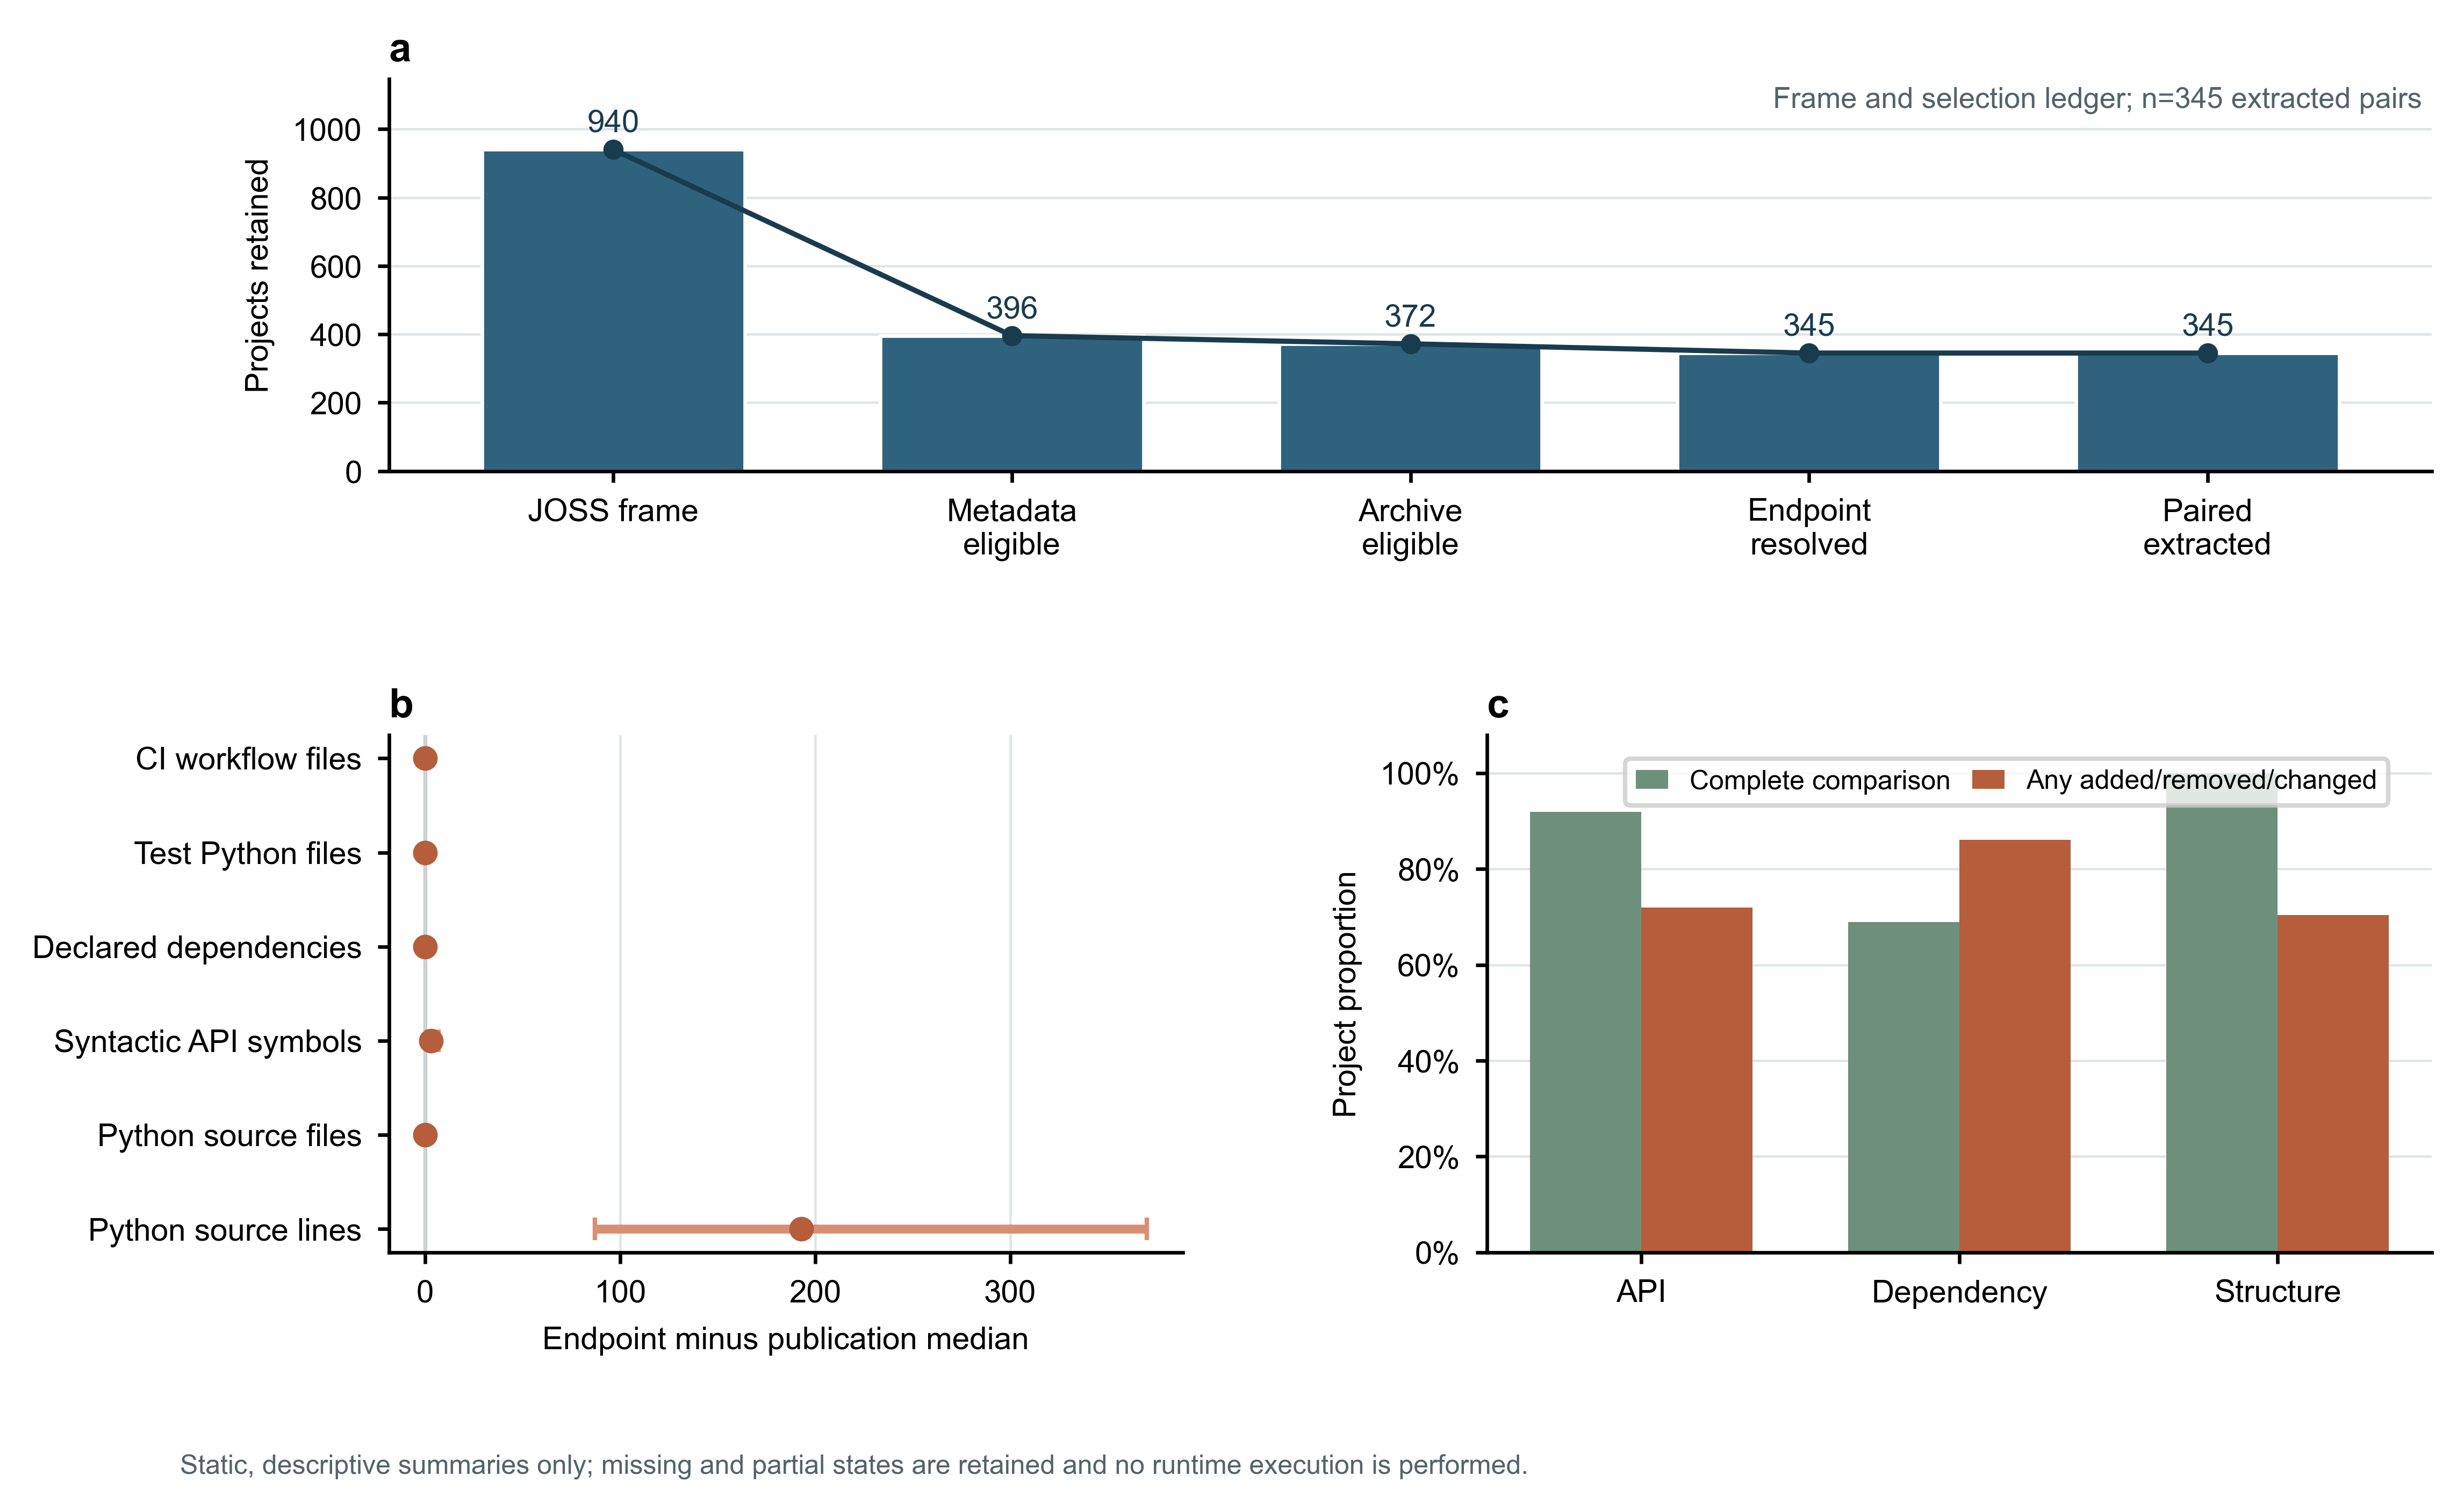
\includegraphics[width=\linewidth]{figures/census_overview.png}
  \caption{\textbf{Selection coverage and static comparison products in the version-paired census.} (a) Attrition from 940 JOSS records to 345 paired projects (396 metadata-eligible; 372 archive-eligible; 27 endpoint-unresolved). (b) Endpoint-minus-publication medians for six static metrics across 345 projects; bars show 95\% percentile intervals from 2,000 project-level bootstrap resamples (seed 20260814). (c) Family-specific proportions with complete parsing and with at least one added, removed or changed feature. Panels report observable static records and selection coverage, not runtime compatibility, software quality, maintenance, impact or population prevalence. Source data are provided with the figure.}
  \label{fig:overview}
\end{figure}

\section{Technical Validation}

\subsection{Archive identity and safety}

All 690 acquired snapshots passed local SHA-256 and archive-member path checks. Publication archives also passed their repository-provided MD5 checks. Endpoint archives are addressed by resolved commit SHAs, and the endpoint ledger preserves the resolution method and evidence URL. The archive validator, schema validator and controlled-vocabulary checks reported no failures. The static pipeline recorded \code{third\_party\_code\_executed=false} in both the extraction manifest and validation records.

\subsection{Parsing completeness and failure retention}

Structure records are complete for all 345 projects at both snapshots. For API records, 322 publication snapshots, 320 endpoint snapshots and 317 paired projects have complete parsing status. Dependency parsing is complete for 250 publication snapshots, 265 endpoint snapshots and 238 paired projects. The remaining states are explicit in the structure and delta tables; no missing value was replaced by zero. The validation table retains 157 expected \code{python\_ast\_parse} errors and 8 \code{api\_source\_read} errors, together with 179 metadata-parse warnings and 1,152 AST warnings. These events are parser limitations to be stratified or excluded by downstream users, not evidence that the source code was executed.

\subsection{Referential integrity and deterministic rerun}

The strict census validator reported PASS for primary-key uniqueness, two-snapshot pairing, referential integrity, controlled vocabularies, archive hashes, path safety, evidence-path relativity and the no-execution assertion. A clean rerun from cached immutable inputs produced byte-identical canonical tables. The released manifests bind the input and output SHA-256 values, enabling a reuser to verify that the seven core tables and summary products correspond to the stated parser version.

As an independent provenance spot-check, a deterministic 20-project sample was reconstructed from the cached archives without importing the extraction implementation. All 40 sampled snapshot archives matched their recorded sizes and SHA-256 values, and all 38 sampled API or dependency evidence paths were found in the corresponding normalized archive member sets. This audit is a bounded reconstruction check rather than a population accuracy estimate; its ledger is released as \code{independent\_reconstruction\_audit.csv} with a machine-readable summary.

\subsection{Selection and endpoint accounting}

The selection ledger accounts for all 940 frame records. The attrition path is retained as data rather than collapsed into a single denominator: 940 screened, 396 metadata-eligible, 372 publication-archive eligible, 345 endpoint-resolved and 345 paired-extracted. The 7 metadata-stage unresolved records, 4 archive-stage unresolved records and 27 endpoint-unresolved records remain visible with reason codes. Consequently, the 345-project paired summaries use the resolved-pair denominator, whereas endpoint-resolution proportions use the 372 archive-eligible denominator when unresolved endpoints are shown.

\section{Usage Notes}

Users can join \code{project\_records.csv} to \code{snapshot\_records.csv} through \code{project\_id}, attach child observations through \code{snapshot\_id}, and join cross-snapshot comparisons through \code{pair\_id}. Analyses of dependency or interface changes should filter or stratify by \code{comparison\_status}; partial and unavailable rows must not be silently treated as complete. Empty cells denote unavailable or inapplicable upstream values, while a recorded zero is a measured zero.

The principal reuse cases are (i) attrition-aware studies of publication-to-repository linkage, (ii) comparison of declared dependency and Python-version metadata parsers, (iii) benchmarking of source-level interface extraction, (iv) analyses of test and CI configuration co-occurring with other static changes, and (v) methods studies of missingness, parser warnings and deterministic data reconstruction. These uses can be implemented from the released tables without rebuilding the complete archive-pairing pipeline. The project and snapshot identifiers also make it possible to join the records to later registry or source-history resources while preserving the original provenance boundary.

The syntactic interface heuristic excludes private names and selected non-source directories but cannot reproduce Python import semantics, dynamic exports, conditional imports or generated interfaces. Syntactic differences require a language- and compatibility-specific interpretation and must not be treated automatically as breaking changes \cite{jayasuriya2025syntactic,mahmud2023android,bogart2021breaking}. Dependency rows describe declarations and do not encode solver results, installed versions or transitive closure; execution-oriented build reproducibility and dependency-error repair remain outside the dataset \cite{mukherjee2021dependency}. Source-line counts, extracted-row volumes and metadata-file presence are not quality, maintenance, sustainability or impact scores. The external scope is limited to JOSS articles in the 2018--2020 frame, repositories meeting the stated GitHub/Python/licence rules and endpoint state resolved on 14 August 2026.

\section*{Data Availability}

The derived dataset will be deposited in \placeholder{formal repository and dataset DOI to be inserted before submission} as version v0.2 under the Creative Commons Attribution 4.0 International licence. The record will contain the seven core tables, schemas, manifests, controlled vocabularies, selection and endpoint ledgers, validation products, figure source data and checksums. This machine-actionable packaging keeps provenance metadata with the research artefacts \cite{soilandreyes2022rocrate}. Source archives are identified at row level by their public archive DOI or immutable Git commit and SHA-256. Anonymous download access must be tested before first-round submission, and the final DOI and repository citation must replace the marked field.

\section*{Code Availability}

The custom code used to construct the frame, resolve endpoints, inspect archives, extract static records, construct deltas, validate tables and generate figures is available from the public GitHub repository \url{https://github.com/bianyanbo44-afk/reprodecay-scidata} and its versioned v0.2.1 release \url{https://github.com/bianyanbo44-afk/reprodecay-scidata/releases/tag/v0.2.1} under the MIT License. The release includes the Python environment, parser version, command sequence, tests and the exact input-hash manifest used for this manuscript. A DOI-minted archival copy will be linked before publication.

\section*{Author Contributions}

\placeholder{CRediT roles for Yanbo Bian and Zhihai Wang to be confirmed before submission.}

\section*{Competing Interests}

The authors declare no competing interests.

\section*{Funding}

This work received no external funding.

\section*{Ethics Statement}

This work uses public scholarly records and public repository metadata and does not involve human participants, private repositories or interaction with contributors. Institutional and rights-review requirements should be confirmed before submission. The release plan excludes raw third-party archives unless redistribution rights are established.

\section*{Acknowledgements}

The authors will acknowledge the public Crossref, JOSS, Zenodo, Figshare and GitHub services used to construct the frame and immutable source links. AI-assisted tools were used for language drafting and code-oriented quality checks; all data-generation decisions, source interpretation and final claims remain the authors' responsibility.

\bibliographystyle{unsrt}
\bibliography{references}

\end{document}
